\chapter{Måling af stemningsleje}\label{maaling_af_stemningsleje}
For at kunne indsamle forstyrrende data om en patient er det nødvendigt at vide hvordan dette på nuværende tidspunkt gøres i psykologien.
Derfor er det blevet undersøgt i litteratur fra psykologien, samt de interviews der er beskrevet i fællesrapporten, hvordan de diagnosticerer og evaluerer patienter. 
Disse metoder vil i dette kapitel blive præsenteret.

\subsection{Positive Affect and Negative Affect Scales (PANAS)}
PANAS er en anerkendt liste af begreber relateret til positiv og negativ affekt, som bruges til at vurdere stemningsleje, som beskrevet i \citet{panas}.

% Baseret på tidligere skalaer, bevist uafhængighed begreberne mellem
% Afprøvet præcision med forskellige tidsintervaller
% Afprøvet præcision vha. test/gentest
% Afprøvet som måling af angst, depression og generelt psykologisk lidelse; God correlation ift. NA og kendte skalaer (dårlig, som forventet, correlation mellem PA og samme skalaer)

PANAS er et forsøg på at lave et skema, med skalaer til positiv og negativ affekt, til brug i forbindelse med estimering af humør.
Den er baseret på tidligere eksisterende skalaer, med et ønske om at lave en mere generel og pålidelig skala.
Dette er gjort ved at udvælge og afprøve en række begreber, hvis pålidelighed, præcision og uafhængighed er sikret gennem en lang række analyser og forsøg.

PANAS skemaet er 2 lister af henholdsvis 10 positive og 10 negative ord (oversat):\\
\begin{center}
\begin{tabular}{r | l}
interesseret & irritabel \\\newline
aktiv & fjendtlig \\\newline
eksalteret & skamfuld \\\newline
inspireret & oprevet \\\newline
stærk & nervøs \\\newline
målbevidst & skyldig \\\newline
opmærksom & bange \\\newline
agtpågivende & anspændt \\\newline
entusiastisk & nødstedt \\\newline
stolt & ræd
\end{tabular}
\end{center}
\bruno{Indsæt original fra artiklen i appendiks.}

Alle tyve vurderes med en værdi fra et til fem som indikerer i hvor høj grad begrebet er oplevet.
Om hvorvidt det er oplevet skal tænkes i forhold til en bestemt tidsperiode; \textit{I øjeblikket, I dag, De seneste par dage, De seneste par uger, Det seneste år, Generelt}.

Præcisionen af skalaerne er afprøvet først og fremmest ved at udfylde skemaet med blik på forskellige tidsperioder nævnt ovenover.
Yderligere for at verificere præcisionen, er skemaet afprøvet med samme person, samme tidsperiode(r) flere gange over en periode på femten uger, hvorefter de besvarelserne sammenlignes med en forventning om jo længere tidsperiode jo bedre sammenhold.

Vigtigst af alt er PANAS også blevet sammenlignet med kendte skemaer der bruges i forbindelse med måling af angst, depression og generel psykisk lidelse.
Her vises god korrelation mellem de skemaer og målene for negative affekt for PANAS.
Og omvendt, som forventet, vises dårlig korrelation mellem skemaerne og målene for positiv affekt.\label{PANAS}

\subsection{Stemningsregistrering}\label{stemningsleje::stemningsregistrering}
Under mødet med Psykolog Janne Rasmussen\cite[Afsnit 1.3, Møde med Psykolog Janne Rasmussen]{faelles} blev der nævnt en metode kaldet stemningsregistrering.
Dette afsnit vil kortfattet beskrive denne metode og dens effekt.

Stemningsregistrering\cite[Appendiks F, Stemningsregistrering]{faelles} hjælper patienten med at reflektere over sin stemningsleje.
Det gør at patienten er mere klar over hvordan han har det.
Stemningsregistrering fungerer som hjælpeværktøj under behandlingen, da det er lettere for behandleren at se hvordan patienten har det vha. stemningsregistreringen og samtidig får patienten selv en bedre forståelse.
Stemningsregistrering fungerer ved at patienten hver dag krydser af i et skema, i det felt der svarer til patientens egen opfattelse af sin stemningsleje.
Dette gør at man kan finde mønstre, fx. at patienten er deprimeret hver søndag.
Dette kan så bruges under samtale med behandleren.
Det eneste krav er at patienten kender sine egne symptomer.

Et eksempel på et skema kan ses på \cref{figure::stemningsregistrerings_skema}.
På skemaet kan patienten udfylde fem punkter:
\begin{itemize}
	\item Stemningsleje
	\item Angst
	\item Antal timers søvn
	\item Medicin
	\item Notater og vægt
\end{itemize}

\begin{figure}
	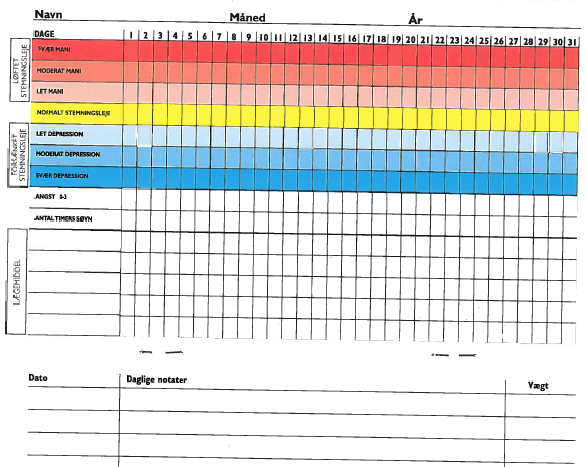
\includegraphics[width=\textwidth]{stemningsregistrerings_skema.png}
	\caption{Et eksempel på et tomt stemningsregistrerings skema.}
	\label{figure::stemningsregistrerings_skema}
\end{figure}

\subsubsection{De fem punkter}
I dette afsnit bliver de fem punkter udspecificeret.
De er baseret på \citet[Appendiks F, Stemningsregistrering]{faelles}.
\paragraph{Stemningsleje}
Under dette punkt er der syv valg:
\begin{itemize}
	\item \textbf{Normal}(gul), hvis der ikke er symptomer på mani eller depression. Energiniveauet er normalt. Søvnen er normal. Forholdsvis nemt at passe daglige aktiviteter.
	\item \textbf{Let mani}(lyserød), hvis patienten føler sig opstemt og optimistisk eller mere irritabel end sædvanligt. Patienten oplever følgende; mere energi, flere ideer, øget selvtillid, mere udadvendt, mere talende, øget sexuallyst, rastløs, sover mindre, vanskeligt ved at arbejde effektivt og fungere socialt.
	\item \textbf{Moderat mani}(mellemrød), griner på upassende tidspunkter eller er meget irritabel og utålmodig, taler meget også selvom andre prøver at sige noget, sover kun fire timer om natten, svært ved at samle sig om en ting, ikke i stand til at passe arbejdet, tænker meget på sex.
	\item \textbf{Svær mani}(rød), ekstatisk, meget grinende eller er vredladen og ofte udskældende, verbale eller fysiske kampe med andre, tror på vedkommende har særlige evner (læse tanker, høre stemmer), konstant bevægelse, sover meget lidt eller ikke, mister kontrollen.
	\item \textbf{Let depression}(lyseblå), lettere trist, selvkritisk, negative tanker, lidt større søvnbehov, svært ved at falde i søvn, træt, er livet værd at leve?, mindre effektiv, kan godt arbejde, andre bemærker det ikke.
	\item \textbf{Moderat depression}(mellemblå), nedtrykt, opgivende, uinteresseret, følger sig langsom, sover mere, svært ved at falde i søvn, bebrejdelse, ukoncentreret, får ikke tingene gjort, selvmordstanker, svært at passe arbejde.
	\item \textbf{Svær depression}(blå), meget nedtrykt, føler intet, håbløshed, energiløs, mistet interessen for alt, ingen appetit, kan ikke sove, alvorlige selvmordstanker, hører stemmer eller ser syner, kan ikke arbejde, svært ved egenomsorg, i sengen det meste af dagen.
\end{itemize}

\paragraph{Angst}
Angst angives på en skala fra og med nul til og med tre.
\begin{itemize}
	\item \textbf{0} svarer til at man ikke oplever nogen form for angst.
	\item \textbf{1} Lettere ængstelig, men påvirker ikke dagligdagen.
	\item \textbf{2} Konstant ængstelig, funktionsniveau påvirkes.
	\item \textbf{3} Udtalt angst, kan næsten ikke foretage sig noget.
\end{itemize}

\paragraph{Antal timers søvn}
Antal timers søvn selvom søvnen har været afbrudt.

\paragraph{Medicin}
Her skrives hvilket og hvor meget medicin der tages i begyndelsen af hver måned.

\paragraph{Notater og vægt} 
Vægten skal registreres mindst en gang om måneden.
Kvinder angiver her de dage de har menstruation.
Andre notater kan være ting som; jobskifte, dødsfald, forelskelse, konflikter osv.

\subsubsection{Information før brug}
Patienten skal oplyses om hvordan han selv finder frem til sit stemningsleje.
Lige nu sker det ved at patienten får udleveret et hæfte som kan ses i \citet[Appendiks F, Stemningsregistrering]{faelles}).
Dette hæfte gennemgås sammen med en psykolog.
Hvis denne metode skal bruges på en mobil platform er det derfor vigtigt at huske at holde dette møde med patienten inden.
Det kan dog også lede op til følgende åbne problemstilling: \textit{Hvordan oplyser vi patienten, om de informationer der er i hæftet, på en mobil platform?}
En mulig løsning kunne være at introducere en gennemgang til første gangs brugere på den mobile platform eller en hjælpe-knap der fortæller om hvert af de fem punkter.

\section{Hamilton Depressionsskala(HAM-D)}
Psykolog Janne Rasmussen fortalte under interviewet at man brugte HAM-D til at afgøre om hvilket depressions stadie man er på.\cite[Afsnit 1.3, Møde med Psykolog Janne Rasmussen]{faelles}
Derfor er HAM-D valgt som en af metoderne til at måle stemningslejet.

HAM-D er en metode oprindeligt udgivet af Max Hamilton \cite{ham_d}, der kan bruges på patienter der tidligere har fået diagnosticeret depression. 
Metoden består af 17 variable faktorer.
Disse variable faktorer giver intervieweren en værdi på 0-4 eller 0-2\footnote{Kommer an på om det er muligt at have et interval på fem eller tre på en given variable faktor.} alt efter hvor meget patienten har symptomet (det maksimale antal point der kan opnås er 52 point).
Intervieweren er en faglig kompetent person indenfor området.
For at gøre det nemmere for intervieweren er de variable faktorer oftest omformuleret til 17 spørgsmål, den danske version kan findes på \citet{ham_d_dansk}.
Når alle værdier er afgivet adderes disse og siger noget om patientens stemningsleje:
\begin{itemize}
	\item \textbf{0-13} ingen depression.
	\item \textbf{13-17} let depression.
	\item \textbf{18-24} moderat depression.
	\item \textbf{25-52} svær depression.
\end{itemize}

Som nævnt foretages HAM-D af en interviewer der er faglig kompetent.
Da spørgsmålene skal præsenteres på en mobil platform lægger det op til følgende åbne problemstilling: \textit{Hvordan præsenteres HAM-D på en mobil platform uden en interviewer?}
En mulighed er at arbejde sammen med en psykolog og en informatiker der sikrer at kommunikere de 17 variable faktorer ud til patienten, så de kan svare på dem.
